\chapter{Metodologia}
\label{c:Metodologia}

%%%%%%%% Crec que la metodologia hauria d'anar desprès dels objecius i començar d'aqeusta forma...

Un cop hem presentat els objectius, ara toca explicar de quina manera els assolirem. Tal i com hem mencionat als objectius, no només és important fer recerca, sinó que hem de fer recerca de qualitat, intentant reproduir la manera en que es fa recerca en els grups d'investigació amb les limitacions pròpies d'un treball de recerca.

En aquest treball el tutor, que ha actuat com el cap del grup de recerca, ha determinat quines eines es fan servir en el grup. Per tant, com a membre del grup m'he hagut d'adaptar a les seves demandes i ha formar-me en l'ús d'aquestes eines. A continuació presentaré aquestes eines i explicaré quines avantatges presenten respecte a altres eines més populars, però que no estan pensades per a l'ús en el camp de la recerca científica.

Per descomptat, a part de la metodologia pròpia del grup de recerca, també hi ha metodologia pròpia de la recerca que es presentaran al capítol~\ref{c:RecercaPrevia}~\nameref{c:RecercaPrevia}.


%Ara agruparia les eines en tres capítols. i afegir molta bibliografia, documenta bé el treball

\section{Entorn col·laboratiu} \label{sec:Entorn Col·laboratiu}

El Git~\cite{git} és un sistema de repositoris que permeten el treball col$\cdot$laboratiu i està especialment dissenyat per als projectes científics. En aquest TR he creat un projecte (TR-KM-2025~\cite{TR-KM-2025}) a
la plataforma GitHub~\cite{GitHub} que ofereix una plataforma per a desenvolupar projectes de codi obert. Aquest entorn permet la traçabilitat i la transferència de coneixement entre la comunitat científica.

% \subsection{GitHub} \label{c:GH}
% Per últim, explicaré més sobre GitHub~\cite{GitHub}, tal com he comentat a~\nameref{sec:Entorn Col·laboratiu}. La plataforma GitHub ofereix un entorn per desenvolupar projectes de codi obert.
% En aquesta secció ampliaré més el tema de GitHub.
%
% \subsection{Què és i per a què serveix exactament?}

GitHub és una plataforma al núvol per allotjar i gestionar projectes de software que utilitzen el sistema de control de versions Git. Permet a desenvolupadors, investigadors i equips col·laborar en un mateix projecte sense perdre l’historial de canvis; això facilita treballar en un entorn molt més senzill, i és la raó principal per la qual tant jo com els meus companys, que tenim el mateix tutor, hem decidit utilitzar aquesta plataforma.

A més, en el món professional, saber utilitzar GitHub ofereix  avantatges quan cal fer un treball en equip o escriure un article conjuntament amb altres persones.

\subsection{Avantatges d’utilitzar GitHub}
\begin{enumerate}
 \item \textbf{Control de versions amb Git:} Desa l’historial complet del projecte, permetent tornar a estats anteriors o revisar qui ha fet cada canvi.
 \item \textbf{Col·laboració en equip:} Diverses persones poden treballar en paral·lel, proposar canvis mitjançant \textit{pull requests} i discutir millores en \textit{issues}.
 \item \textbf{Accessibilitat i disponibilitat:} En estar al núvol, pots accedir als teus projectes des de qualsevol lloc i dispositiu.
 \item \textbf{Transferència de coneixement:} Els projectes públics permeten que altres usuaris construeixin, reportin errors o suggereixin millores.
\end{enumerate}

\textit{\textbf{Fonts:}} \cite{GH}



\section{Sistema operatiu}
Per fer un treball més professional i molt més complex, vaig decidir, amb l’ajuda del meu tutor, fer-lo utilitzant un sistema operatiu diferent a l'habitual, però primer vaig haver de triar entre treballar amb una màquina virtual o no.


\subsection{Què és un sistema operatiu?}
\textit{`Els sistemes operatius (tambè anomenats nuclis o kernels) són un conjunt de programes informàtics que fa de \textbf{cervell del teu ordinador}, gestionant els seus recursos físics (hardware), com el processador, la memòria i els perifèrics, i els programes (software), per permetre l'execució d'aplicacions i facilitar la interacció entre l'usuari i la màquina.`}  ~\cite{EE}

% \section{Màquina virtual} \label{sec:mv}
\subsection{Què és una màquina virtual (VM)?}
Una màquina virtual és un entorn informàtic que funciona com un sistema aïllat amb la seva pròpia CPU (Unitat Central de Processament), memòria, interfície de xarxa i emmagatzematge, el qual es crea a partir del hardware.

% \textit{\textbf{Hardware:}} Són tots els components físics d’un sistema informàtic, és a dir, les parts tangibles que es poden veure i tocar.

Les màquines virtuals utilitzen software en un ordinador físic (host) per replicar o emular la funcionalitat d’un ordinador diferent. En resum, una màquina virtual és un ordinador simulat dins d’un ordinador real.

Les màquines virtuals funcionen igual que els ordinadors normals: tenen un sistema operatiu, emmagatzemen fitxers i executen programes.

\subsubsection{Tipus de màquines virtuals}
Les VM poden tenir diferents tasques en funció del tipus de màquina virtual utilitzada.
\begin{enumerate}
 \item \textbf{Màquina virtual de procés}: Serveix per executar un programa com si fos natiu, sense importar el sistema operatiu o el hardware real. No instal·la un sistema operatiu complet, sinó que permet executar programes d’una altra plataforma.

 \textbf{Avantatges:}
 \begin{enumerate}[1)]
  \item Consumeix pocs recursos (RAM i CPU) comparat amb un sistema operatiu complet.
  \item Pots executar programes en qualsevol sistema operatiu compatible.
  \item Si falla, no afecta el sistema operatiu principal.
 \end{enumerate}
 \textbf{Desavantatges:}
 \begin{enumerate}[1)]
  \item Només funciona per a un tipus de programa o plataforma específica (ex. Java).
  \item No pots executar un sistema operatiu complet, només aplicacions.
  \item Accés limitat al software: no pot utilitzar tot el potencial del PC.
 \end{enumerate}

 \item \textbf{Màquina virtual de sistema}: Serveix per emular un sistema operatiu complet dins d’un altre; per exemple, pots tenir Linux dins de Windows, o Windows dins de Linux.

  \textbf{Avantatges:}
 \begin{enumerate}[1)]
  \item Permet executar un sistema operatiu complet dins d’un altre.
  \item Pots provar diferents sistemes operatius sense tocar el PC real.
  \item Cada màquina virtual està aïllada, així que errors o virus no afecten el sistema principal.
 \end{enumerate}
 \clearpage
 \textbf{Desavantatges:}
 \begin{enumerate}[1)]
  \item Consumeix molts recursos: necessita RAM, CPU i espai al disc.
  \item Pot ser més lenta que usar un sistema operatiu natiu.
  \item Configurar i mantenir diverses màquines virtuals pot ser més complex.
 \end{enumerate}
\end{enumerate}

\subsection*{Finalment, quina ha estat la tria?}
Degut a la tipologia del meu ordinador personal no he utilitzat cap màquina virtual, l'eina que he utilitzat és \textbf{Xubuntu}, un sistema operatiu basat en \textit{Linux}. Abans de presentar els avantatges de Linux, mostraré una breu comparativa entre Linux i Windows.

\subsubsection{Comparativa Windows vs Linux}
Si volem elaborar una comparativa en Windows i Linux cal fer una llista dels avantatges i dels desavantatges que presenten cadascun. En general, ambdós destaquen \textbf{compatibilitat amb pràcticament tot el hardware}.
% Això és degut al fet que la majoria d’usuaris utilitzen Windows, i per aquest motiu la majoria de proveïdors de hardware fabriquen controladors per a Windows.

En Windows també cal destacar la \textbf{facilitat d’ús} i el \textbf{suport de software}. Aquest últim punt és perquè Windows té una gran audiència, per això els desenvolupadors prefereixen crear jocs i software per a aquest sistema operatiu, donant-li una major optimització, però aquest software no és lliure com en el cas de Linux.

No només parlaré dels punts positius de Windows, sinó també presentaré alguns desavantatges que pot tenir, com ara els \textbf{atacs de virus elevats}. La raó principal és que els `pirates informàtics` poden trencar fàcilment la seguretat de Windows, per la qual cosa els usuaris d’aquest sistema depenen del software antivirus, que requereix pagaments mensuals per protegir-se. En canvi Linux ofereix un alt nivell de seguretat sense cap cost. A més permet la total configuració del sistema per part de l'usuari.

Windows presenta un \textbf{alt consum de recursos informàtics} afavorint el fenomen de l'obsolescència programada. Per exemple, si estàs instal·lant el sistema operatiu Windows, l’ordinador ha de tenir una gran capacitat de RAM, una targeta gràfica potent i molt d’espai al disc dur. Els sistemes operatius Linux funcionen perfectament amb pocs recursos. Aquest punt va ser crucial en tria del sistema operatiu.

\textit{\textbf{Fonts:}}~\cite{AS}
% \section{Xubuntu}
% \subsection{Què és Xubuntu?}
% \subsection{Quin sistema operatiu he triat?}
%
% Per aquest treball he utilitzat \textit{Xubuntu}~\cite{xubuntu}, una distribució del sistema operatiu Linux.
% L’\textbf{Ubuntu} és un sistema operatiu basat en \textit{Linux}.\\

\subsection*{Per què vaig escollir Xubuntu?}
La principal raó és perquè Ubuntu és gratuït i de codi obert; això fa que sigui accessible per a tothom. Té una gran comunitat, cosa que fa que sigui fàcil trobar ajuda i, per últim, perquè és fàcil d’utilitzar per a principiants.





Xubuntu va ser llançat a l’octubre de 2004 per Canonical. Està basat en Linux i deriva de Debian. Xubuntu és de codi obert, cosa que significa que tant el sistema com les seves aplicacions estan disponibles per ser estudiades sense cap cost.

`\textbf{Linux} és un sistema operatiu de codi obert creat per Linus Torvalds l’any 1991, que funciona com una alternativa gratuïta i modificable a sistemes com Windows i macOS~\cite{RH}.

\subsection*{Per a què serveix Xubuntu?}
Hi ha una infinitat de propòsits, però els que més destaquen són els que descriuré a continuació:
\begin{enumerate}
 \item \textbf{Navegar per internet:} Inclou navegadors com Firefox, optimitzat.
 \item \textbf{Programar i desenvolupar software:} És molt utilitzat per desenvolupadors gràcies a la seva compatibilitat amb una infinitat d’eines de desenvolupament.
 \item \textbf{Utilitzar aplicacions d’oficina:} LibreOffice, Thunderbird o GIMP estan disponibles i són fàcils d’instal·lar.
 \item \textbf{Servidors web i bases de dades:} Ubuntu és la distribució de Linux més popular per a hosting i servidors al núvol.
 \item \textbf{Educació i tasques acadèmiques:} Moltes institucions i escoles l’empren per la seva gratuïtat.
 \item \textbf{Substituir Windows en ordinadors antics:} Consumeix pocs recursos comparat amb el SO de Microsoft, cosa que permet prolongar la vida útil del hardware.
\end{enumerate}

\textit{\textbf{Fonts:}} \cite{GD}





% Hi ha moltes més avantatges i desavantatges, però no les puc anomenar totes, ja que això donaria per fer un altre treball de recerca.



\section{Processador i editor de text} \label{sec:Kile}
%%%%%%%%%%%%%%%%%%%%%%%%%%%%%%%%%%%%%%%%%%%%%%%%%%%%%%%%%%%%%%%%%%%%%

% Per explicar la part de metodologia, hauré d'explicar molta informació relacionada amb la informàtica, i intentaré explicar-ho tot de manera que es pugui entendre. Després d’aquesta explicació informàtica, procediré a explicar els materials que utilitzo en els experiments de la part pràctica d’aquest treball.
% \vspace{0.3truecm}
%
% Per explicar la part de metodologia, hauré d’explicar molta informació relacionada amb la informàtica, i intentaré explicar-ho tot de manera que es pugui entendre. Després d’aquesta explicació informàtica, procediré a explicar els materials que utilitzo en els experiments de la part pràctica d’aquest treball.\\
%
% Explicaré la informació de manera clara; el primer punt que explicaré és sobre les màquines virtuals.


% \section{LaTeX} \label{sec:latex}
LaTeX~\cite{LaTeX} és un sistema de composició de text orientat a la creació de documents escrits que presentin una alta qualitat tipogràfica. Però, com funciona aquesta eina i quina utilitat té?

LaTeX és un processador de text d’accés lliure i gratuït que actualament s’utilitza àmpliament en molts sectors de la recerca científica. En aquesta eina l’autor s’ha de centrar només en el contingut del que escriu, en lloc de la presentació visual. L’autor especificarà l’estructura lògica utilitzant conceptes familiars com: capítol, secció, taula, figura, etc., deixant que el sistema LaTeX s’ocupi de la presentació visual d’aquestes estructures.

\textit{\textbf{Fonts:}} \cite{CH}
% \subsection{Avantatges i Desavantatges}
\subsection*{Per què vaig decidir aprendre LaTeX?}
Hi ha molts arguments del motiu pel qual vaig decidir aprendre i utilitzar LaTeX. Un dels motius principals va ser gràcies al meu tutor del treball, que ens va parlar dels molts avantatges que té, i que és una eina estàndard en l’àmbit acadèmic i científic. Aprendre-la ara ens ajudarà molt en el futur, quan haguem de fer més treballs científics. A més, gestiona de manera senzilla fórmules matemàtiques, bibliografies i referències, i vaig considerar que m’ajudaria en el meu desenvolupament acadèmic i professional.

Per tal d'editar un text en LaTeX cal un editor específic. Per al meu TR he triat l'editor de text per a LaTeX Kile.

% He utilitzat aquestes eines per poder elaborar la memòria d'aquest treball. A continuació, explicaré en que consisteixen i quines raons em va impulsar a la seva tria.


% \subsubsection{Què és exactament?}
Kile és un editor de \textbf{TEX/LaTeX integrat} que va ser creat per la comunitat de KDE. Permet crear, compilar i previsualitzar documents LaTeX en una interfície gràfica, i també té mecanismes de previsualització interactius per veure immediatament els resultats de l’edició.

\textbf{Característiques:}
\begin{enumerate}
 \item Compila, converteix i mostra el document amb un sol clic.
 \item Les plantilles i els assistents fan que sigui molt poca feina començar documents nous.
 \item Inserció fàcil de moltes etiquetes i símbols estàndard, amb l’opció de definir (amb un nombre arbitrari) etiquetes personalitzades per l’usuari.
 \item Cerca directa i inversa: podeu clicar en el visualitzador DVI i saltar a la línia LaTeX corresponent de l’editor, o saltar des de l’editor a la pàgina corresponent en el visualitzador.
 \item La cerca de capítols o seccions és molt senzilla: Kile construeix una llista de tots els capítols i seccions del document. Podeu usar la llista per saltar a la secció corresponent.
 \item Permet reunir documents relacionats dins d’un projecte.
 \item Inserció senzilla de cites i referències quan es treballa amb projectes.
 \item Sistema de construcció flexible i intel·ligent per compilar els documents LaTeX.
 \item QuickPreview: vista prèvia d’una part seleccionada del document.
 \item Accés fàcil a diverses fonts d’ajuda.
 \item Edició avançada d’ordres.
\end{enumerate}
\textit{\textbf{Fonts:}}  \cite{KDE} i \cite{kile}

\subsubsection*{Per què vaig escollir Kile}
Vaig escollir Kile perquè ofereix un entorn integrat que permet editar, compilar i visualitzar documents en un sol lloc. És ideal per a projectes llargs gràcies a la seva gestió de múltiples fitxers.
A més, compta amb autocompletat, assistents, símbols matemàtics i cerca inversa, cosa que agilitza molt la feina acadèmica. En ser lliure, gratuït i altament configurable, resulta més complet que els editors bàsics.

% Després de l’explicació de Kile, a mesura que investigava també vaig descobrir que existeixen altres eines que milloren la productivitat acadèmica i professional; una d’elles són les \textbf{màquines virtuals} \ref{sec:mv}.

\vspace*{2truecm}
\hrule
\vspace*{1truecm}

%%%%%%%%%%%%%%%%%%%%%%%%%%%%%%%%%%%%%%%%%%%%%%%%%%%%%%%%%%%%%%%%%%%%%%%%%%%%%%%%%%%%
Aquí finalitza la descripció de la metodologia referent als recursos informàtics triats. Degut a la limitació de pâgines d'un TR no he pogut explicar detalladament alguns dels conceptes presentats a la part d'informàtica. Podeu trobar una explicació més detallada a \nameref{a:metodologia_informàtica}.
%%%%%%%%%%%%%%%%%%%%%%%%%%%%%%%%%%%%%%%%%%%%%%%%%%%%%%%%%%%%%%%%%%%%%%%%%%%%%%%%%%%%


\clearpage

% Després d’això, procediré a explicar el capítol ~\ref{c:RecercaPrevia} ~\nameref{c:RecercaPrevia}.

\section{Recursos de laboratori} \label{s:recursos}
En aquesta secció es descriu la metodologia seguida per dur a terme la part pràctica del treball, centrada en l’anàlisi de la qualitat de l’aigua mitjançant tires reactives. Atès que no disposem d’un laboratori completament equipat, hem creat un petit entorn experimental amb els recursos disponibles, adaptant els materials i les eines a les limitacions que teníem.

Es detallen els materials utilitzats, com les diferents tires reactives per mesurar paràmetres químics i biològics, recipients per a les mostres d’aigua, pipetes, gots de mesura i altres instruments bàsics de laboratori. Aquest enfocament ens ha permès desenvolupar els experiments de manera segura i controlada, tot i les restriccions de recursos.

\begin{enumerate}
 \item
  Tires reactives comprades a Amazon~\cite{tiresReactives}. Les tires reactives són petits trossets de paper o plàstic impregnats amb substàncies químiques que canvien de color quan entren en contacte amb certs components presents en l’aigua. S’utilitzen per mesurar de manera ràpida i senzilla diferents paràmetres químics, com ara el pH, la duresa, els nitrats o el clor.

  \begin{minipage}[h]{0.45\textwidth}
  \begin{figure}[H]
      \centering
      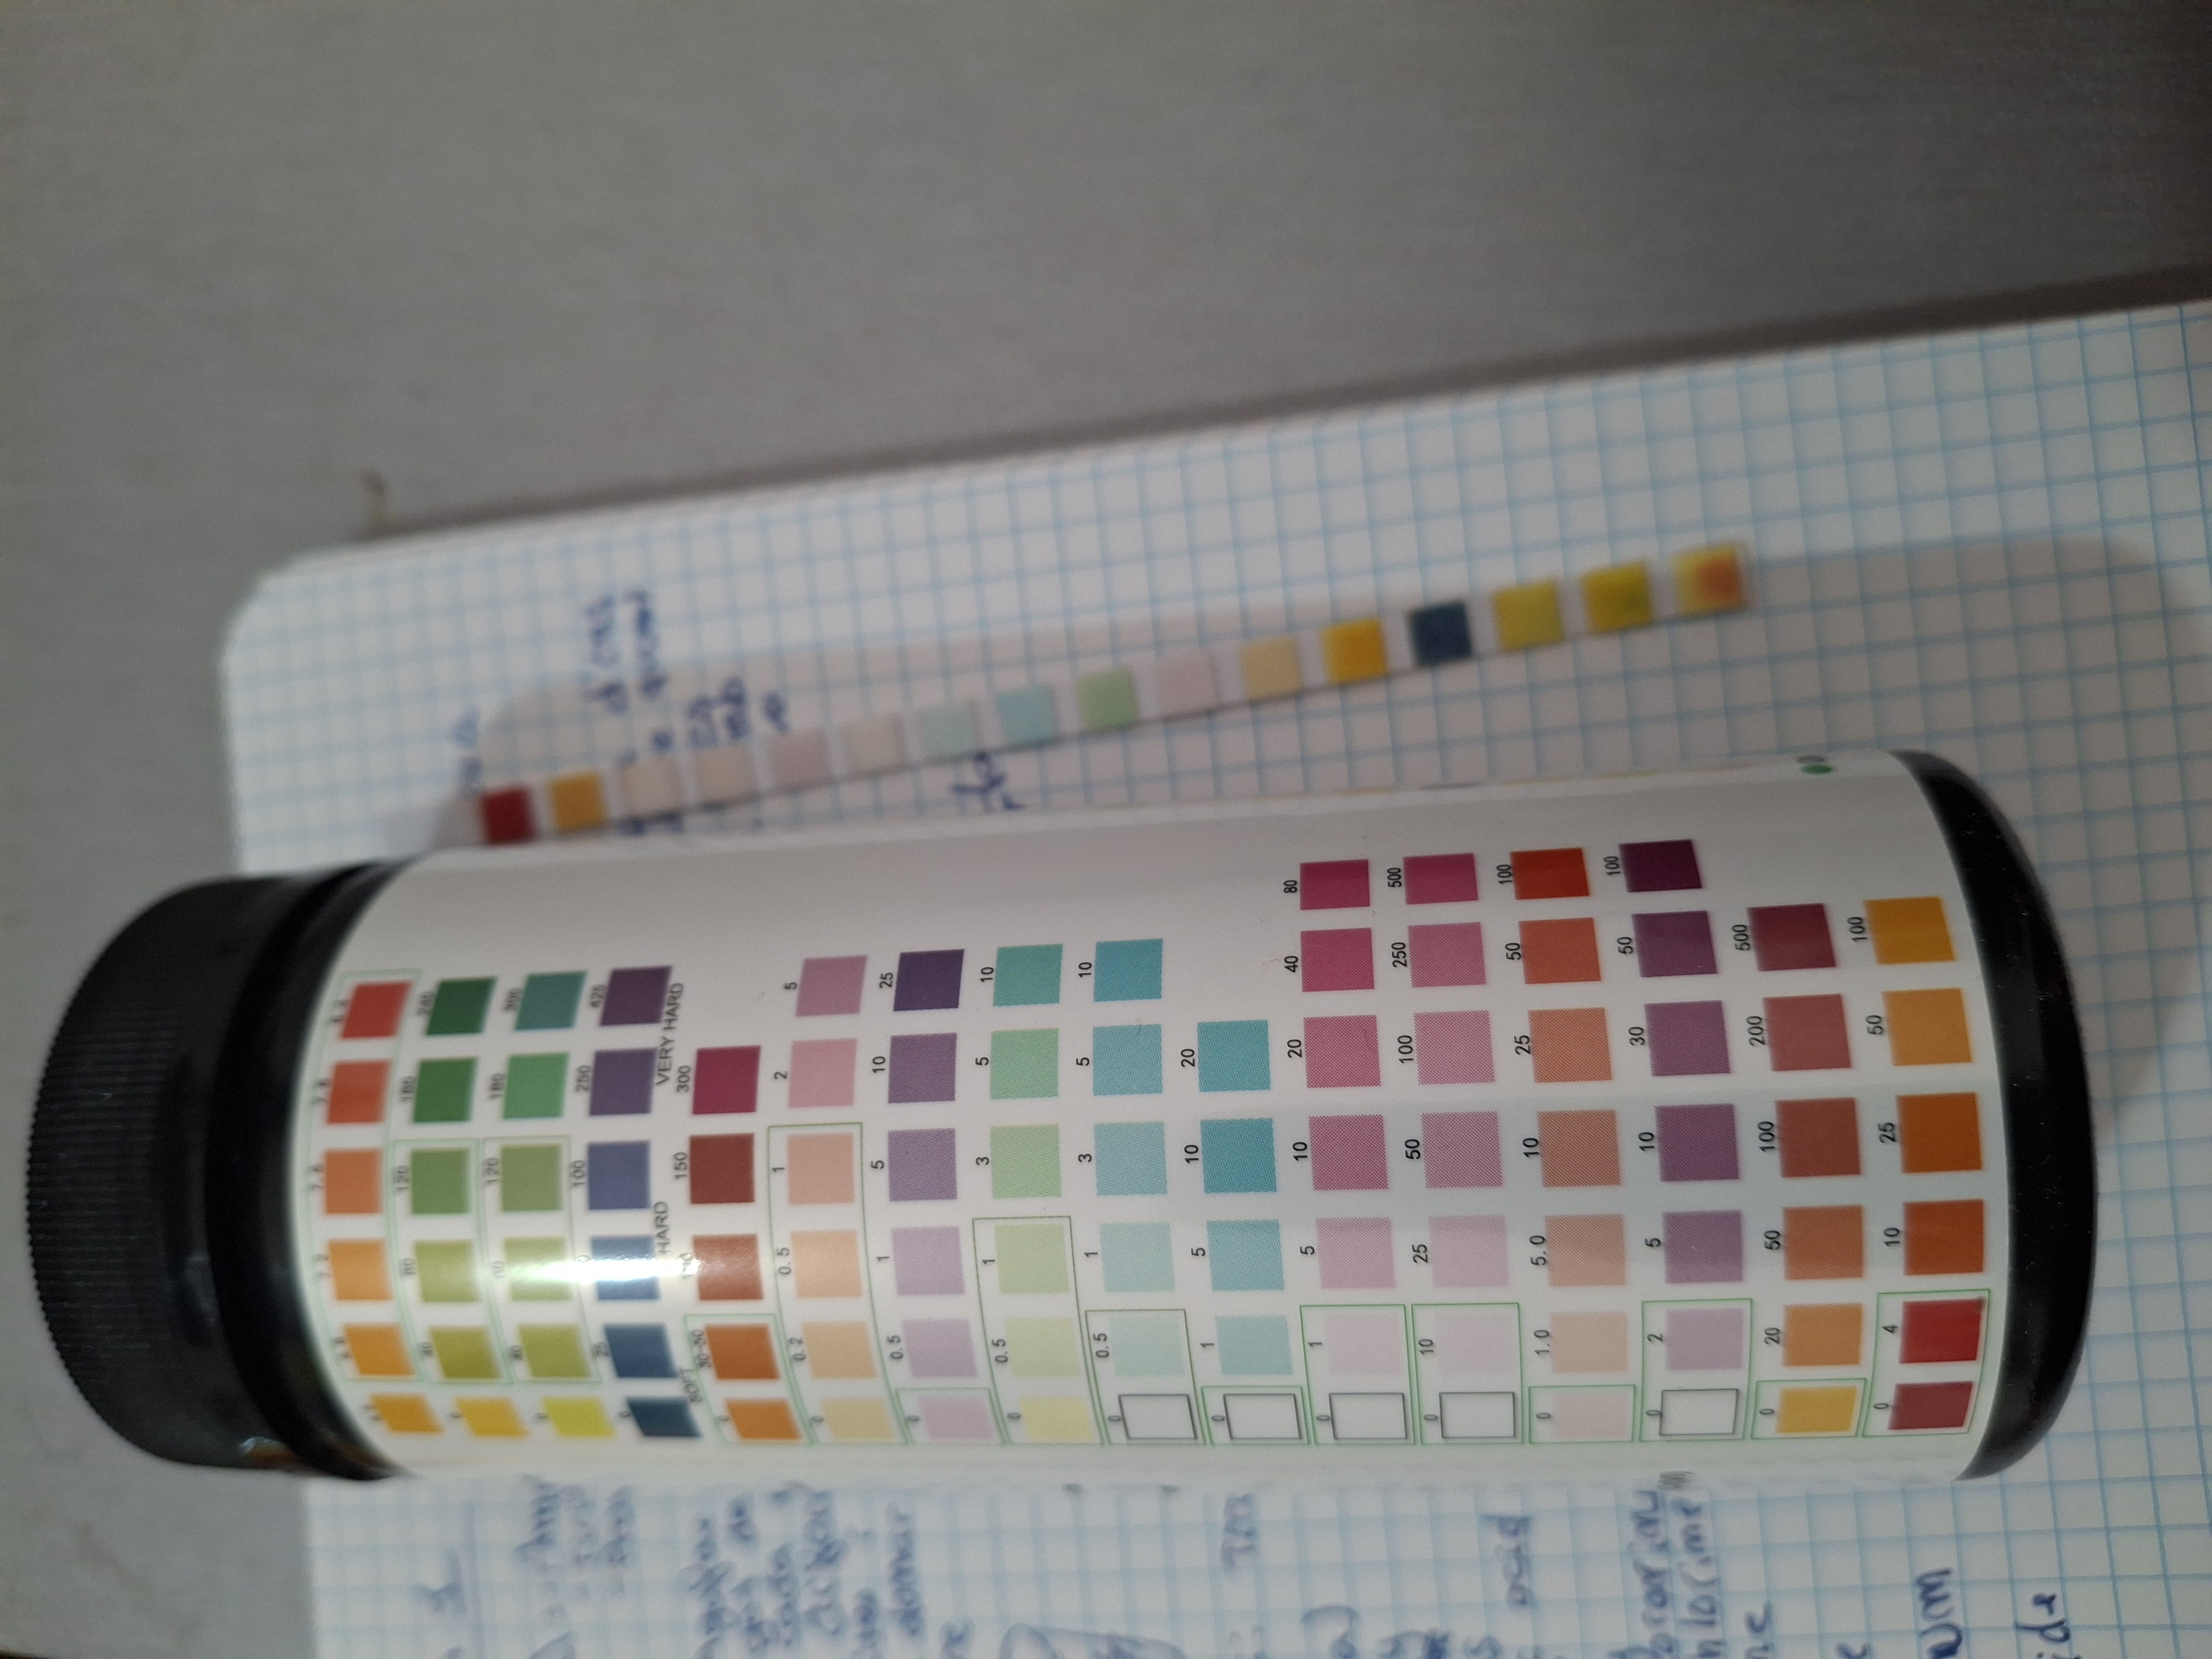
\includegraphics[width=1\textwidth, angle=270]{./Figures/TIres.png}
      \caption{Tires Reactives}
      \label{fig:TiresReactives}
    \end{figure}
  \end{minipage}
  \begin{minipage}[h]{0.45\textwidth}
    \begin{figure}[H]
    \centering
    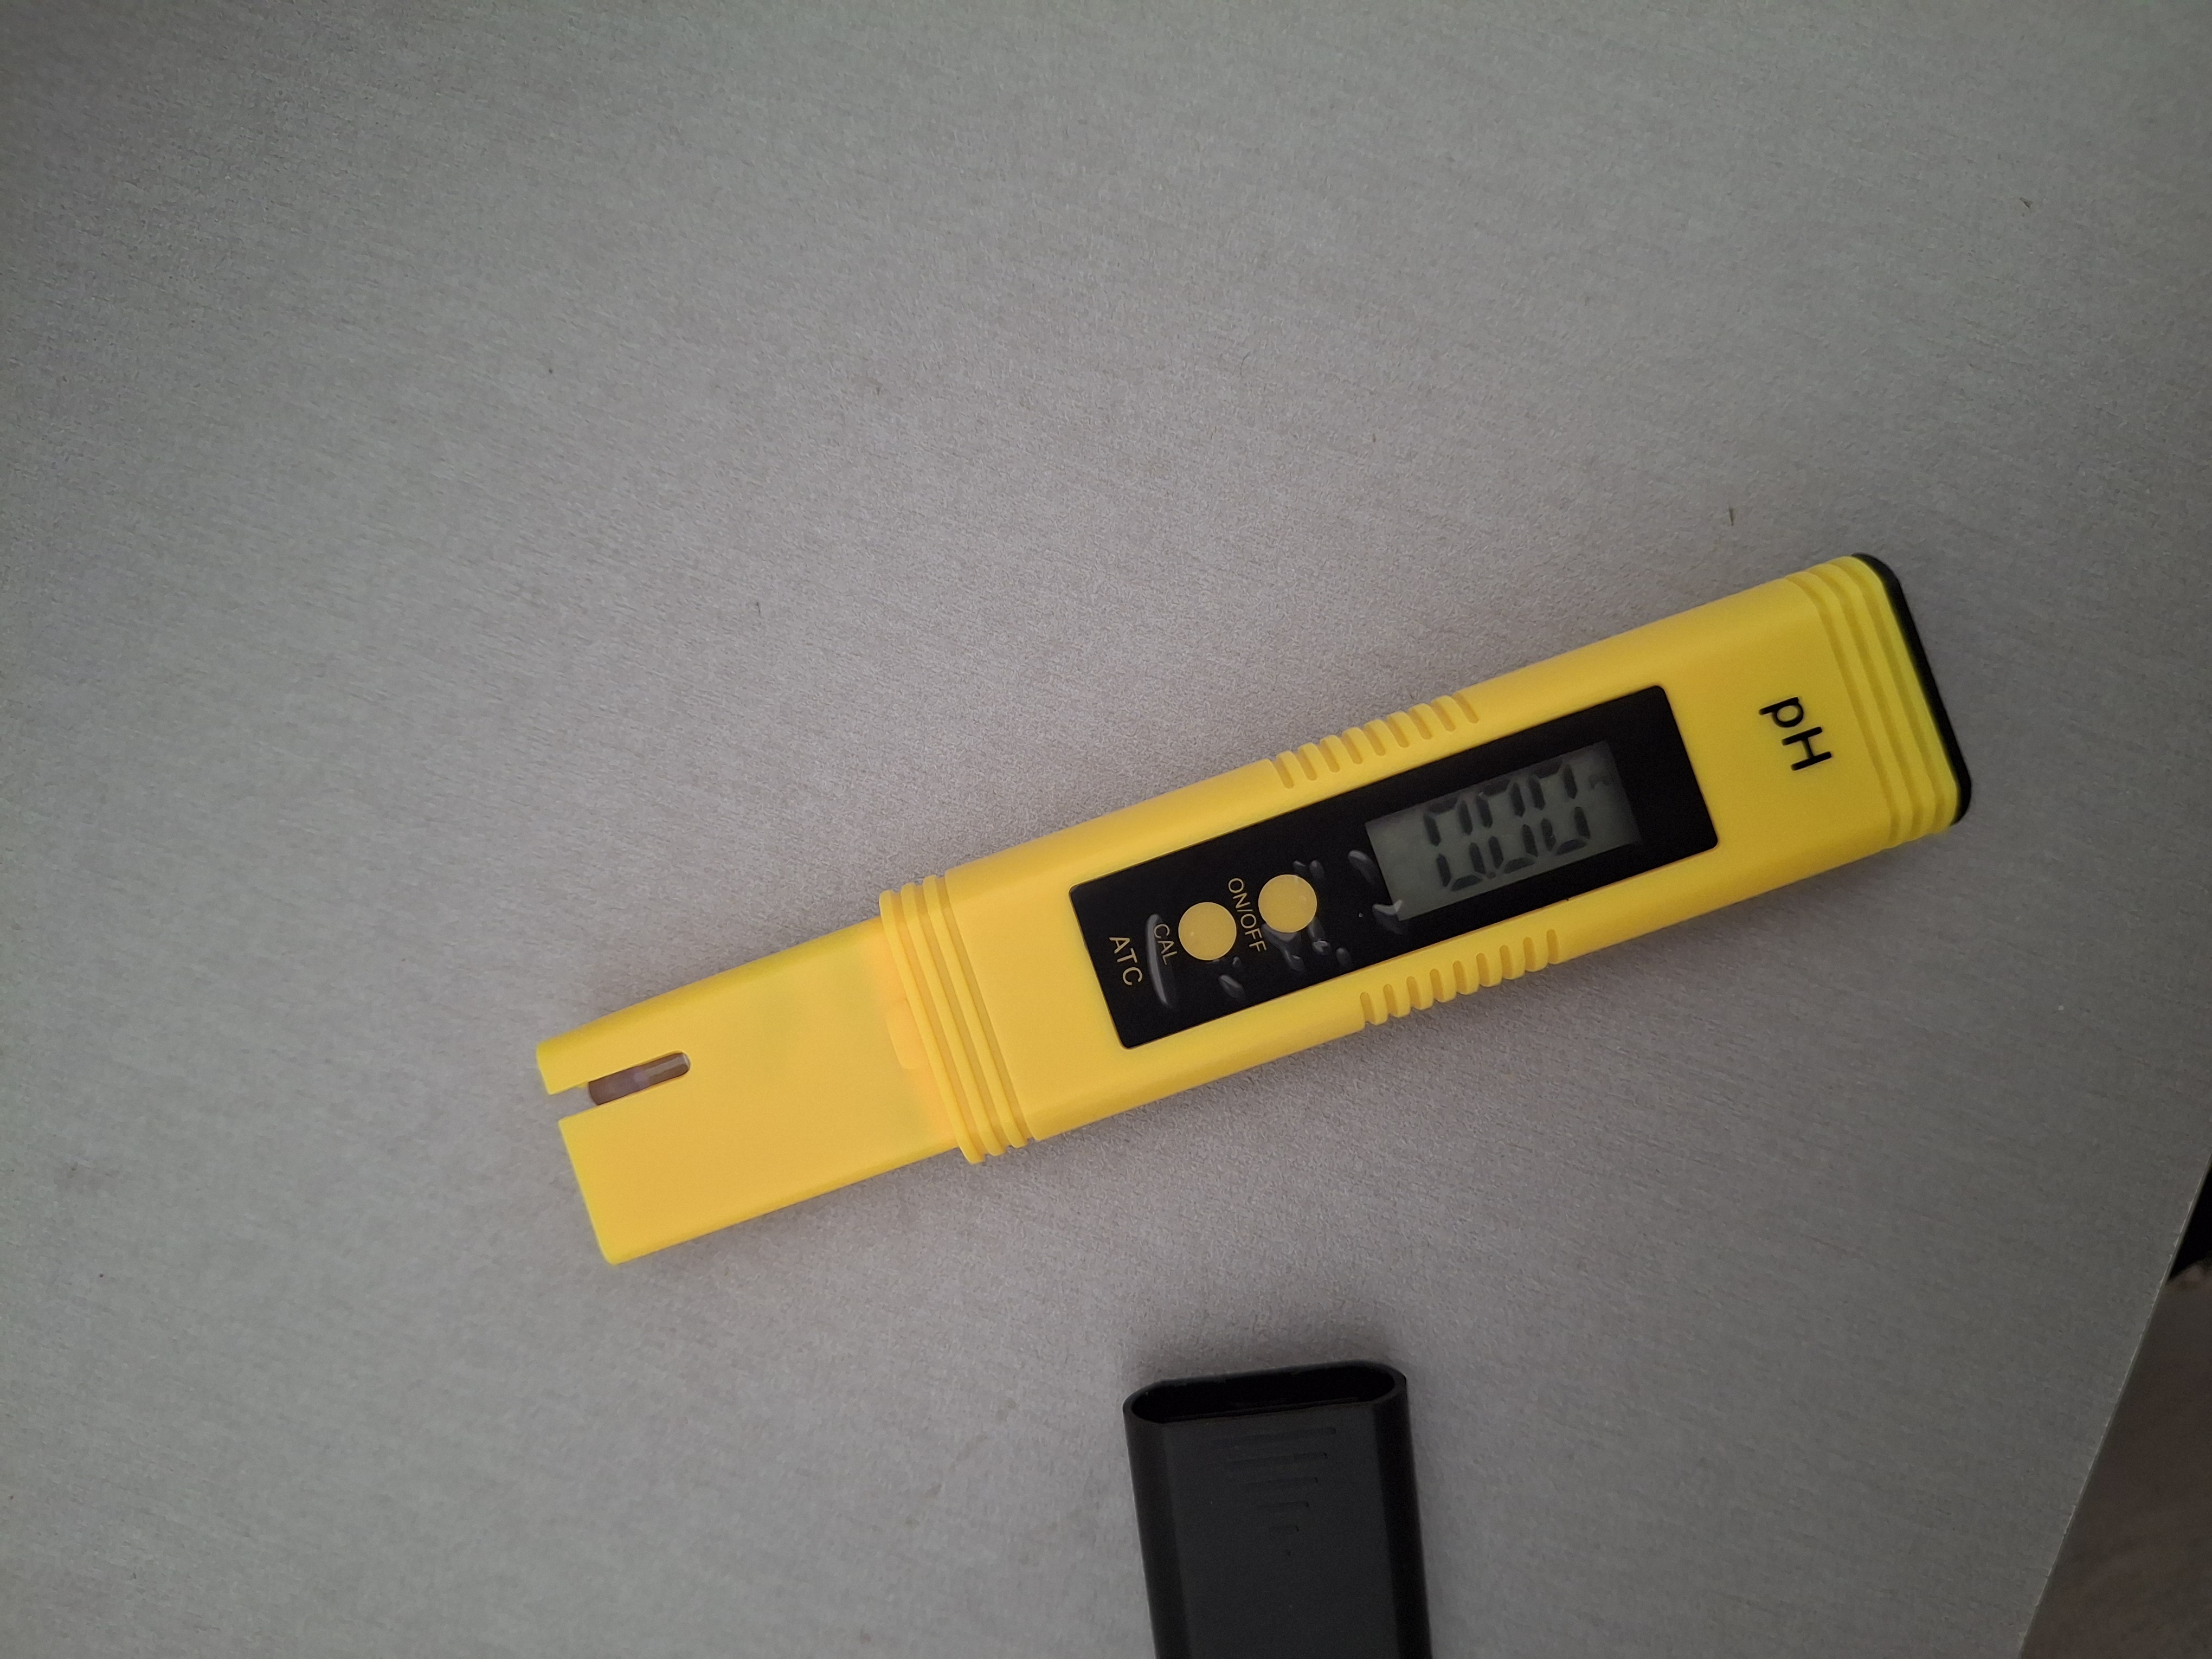
\includegraphics[width=1\textwidth]{./Figures/mesurador.png}
    \caption{Mesurador de pH}
    \label{fig:fotoMesuradorPH}%%%Els labels han de ser tots diferents.
    \end{figure}
  \end{minipage}

%     \begin{figure}[h]
%     \centering
%     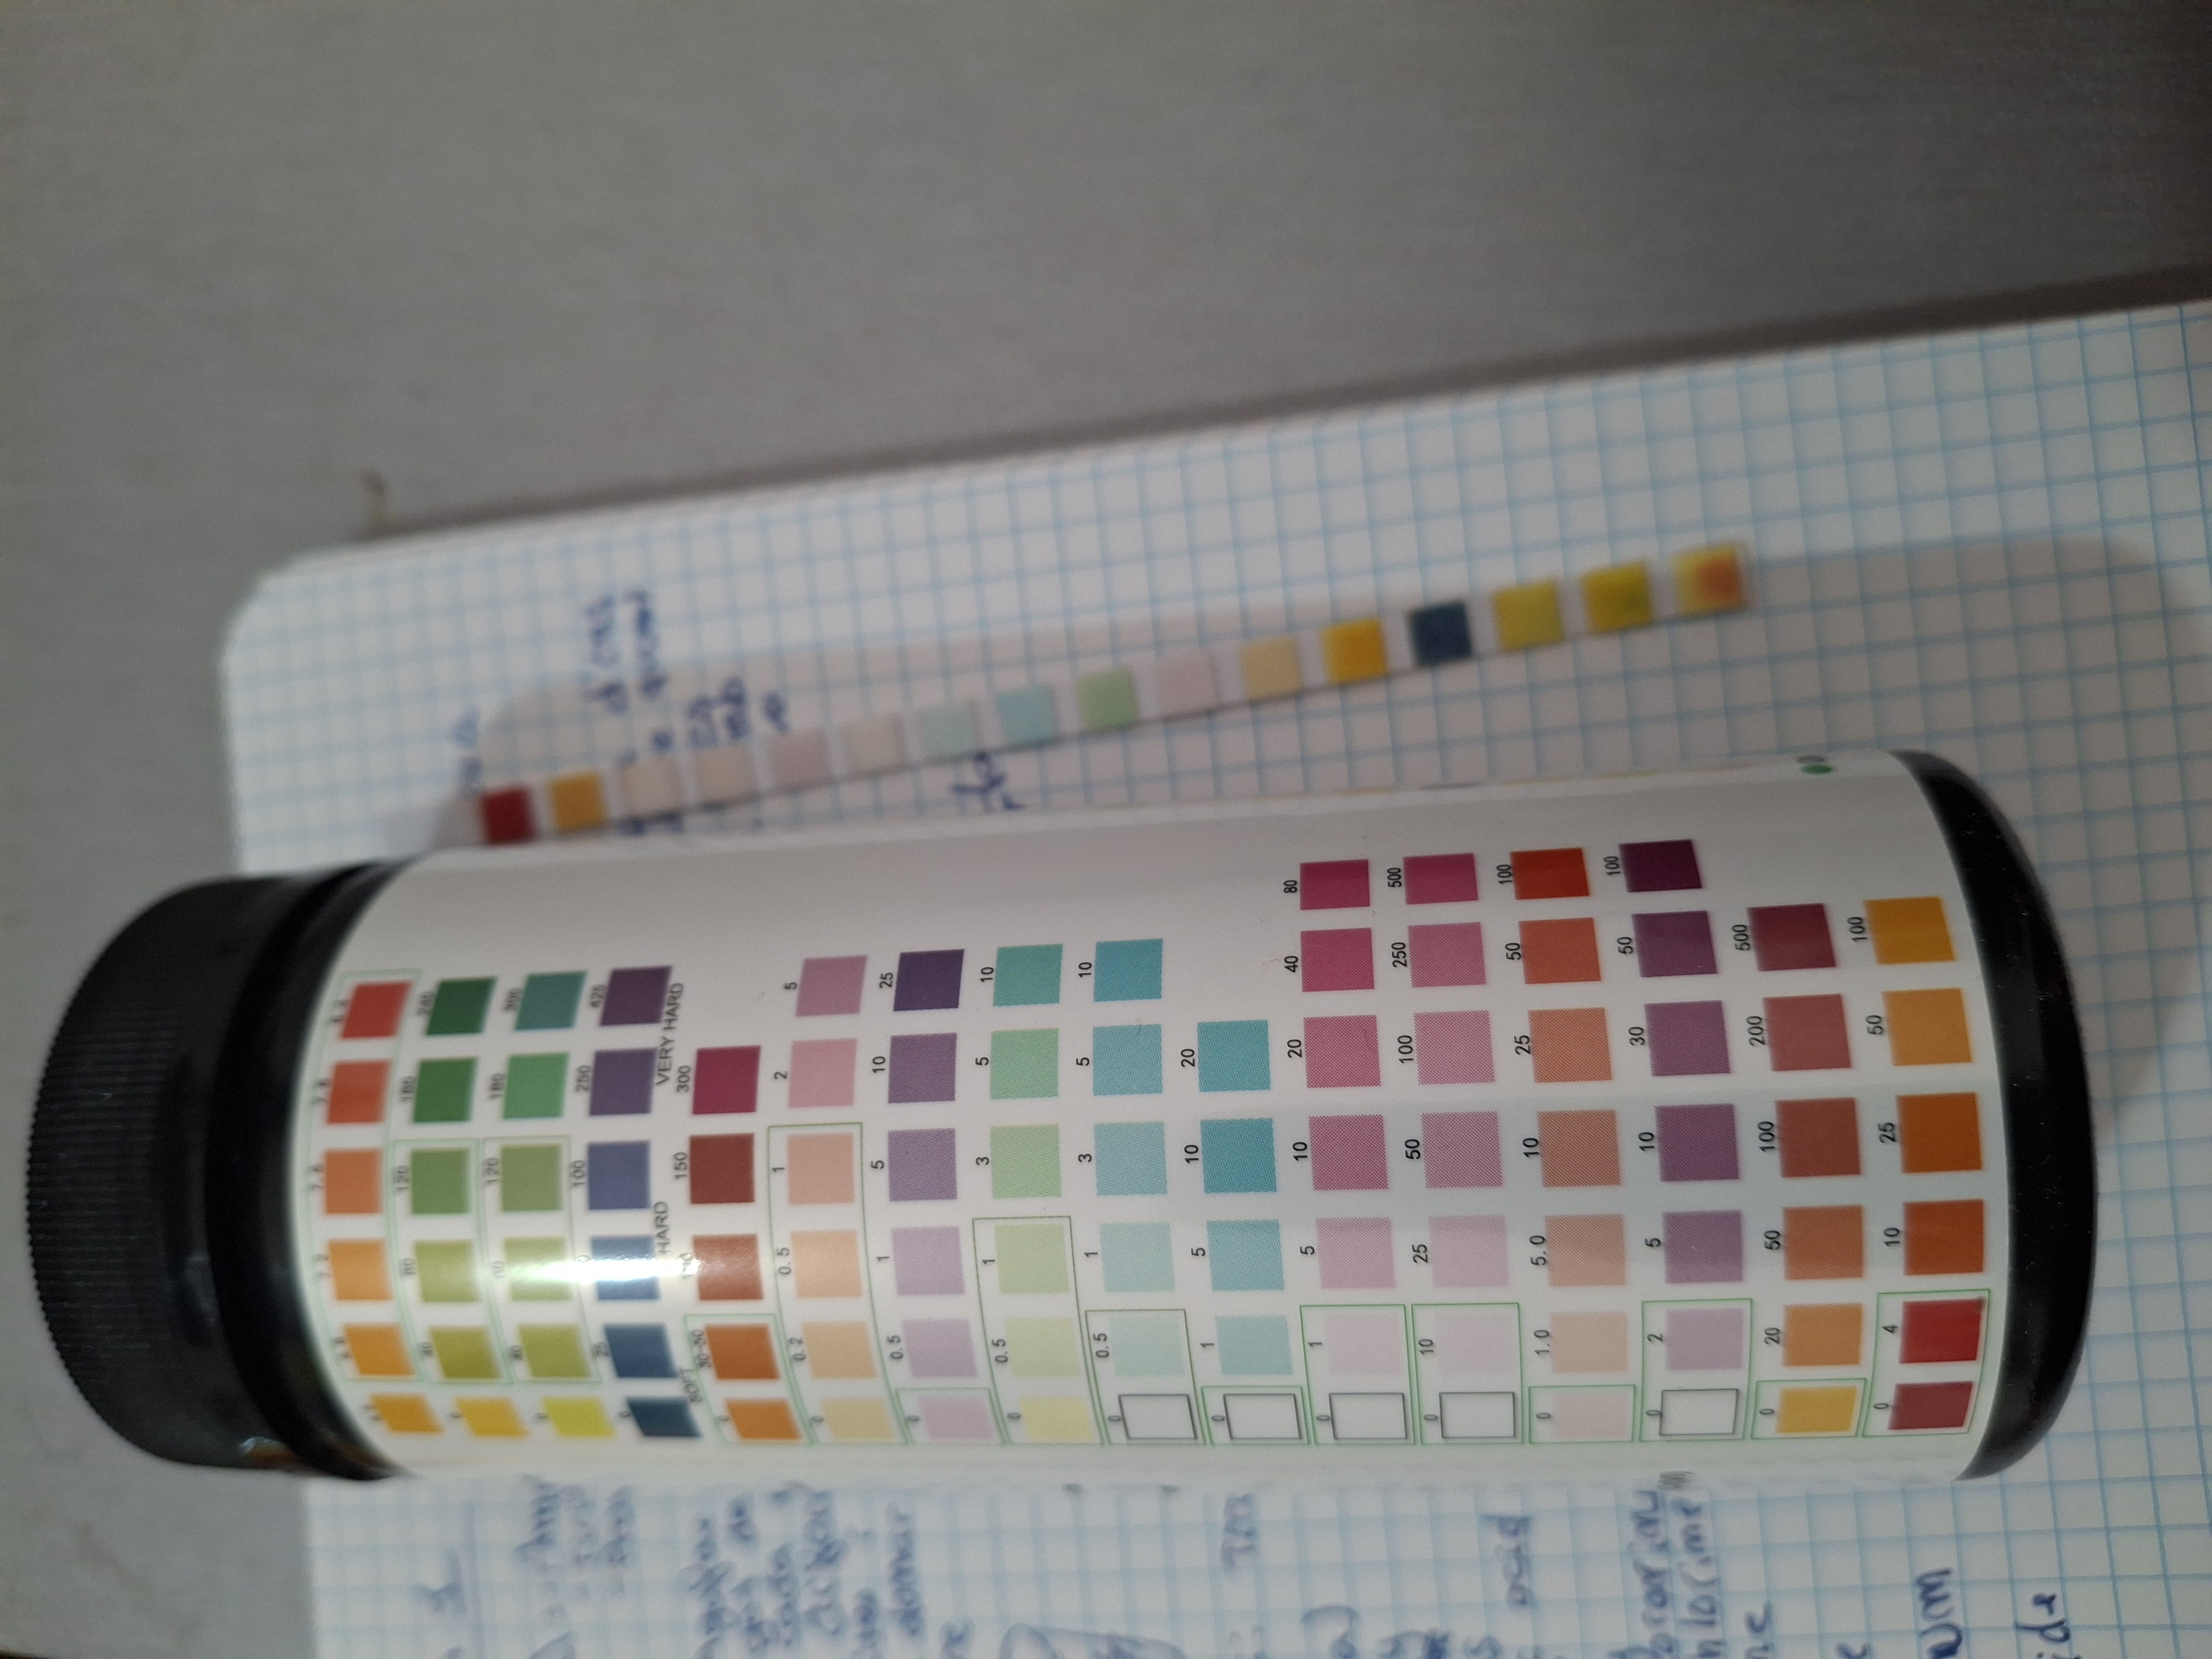
\includegraphics[width=0.5\textwidth, angle=270]{./Figures/TIres.png}
%     \caption{Tires Reactives}
%     \label{fig:TiresReactives}
%   \end{figure}

\item Un mesurador digital de pH cedit pel centre.  El mesurador de pH és un instrument utilitzat per determinar l’acidesa o alcalinitat d’una mostra d’aigua. Mesura la concentració d’ions d’hidrogen (H$^+$) i proporciona un valor numèric que indica si l’aigua és àcida (pH $<$ 7), neutra (pH = 7) o bàsica (pH $>$ 7).
%  \begin{figure}[h!]
% \centering
% 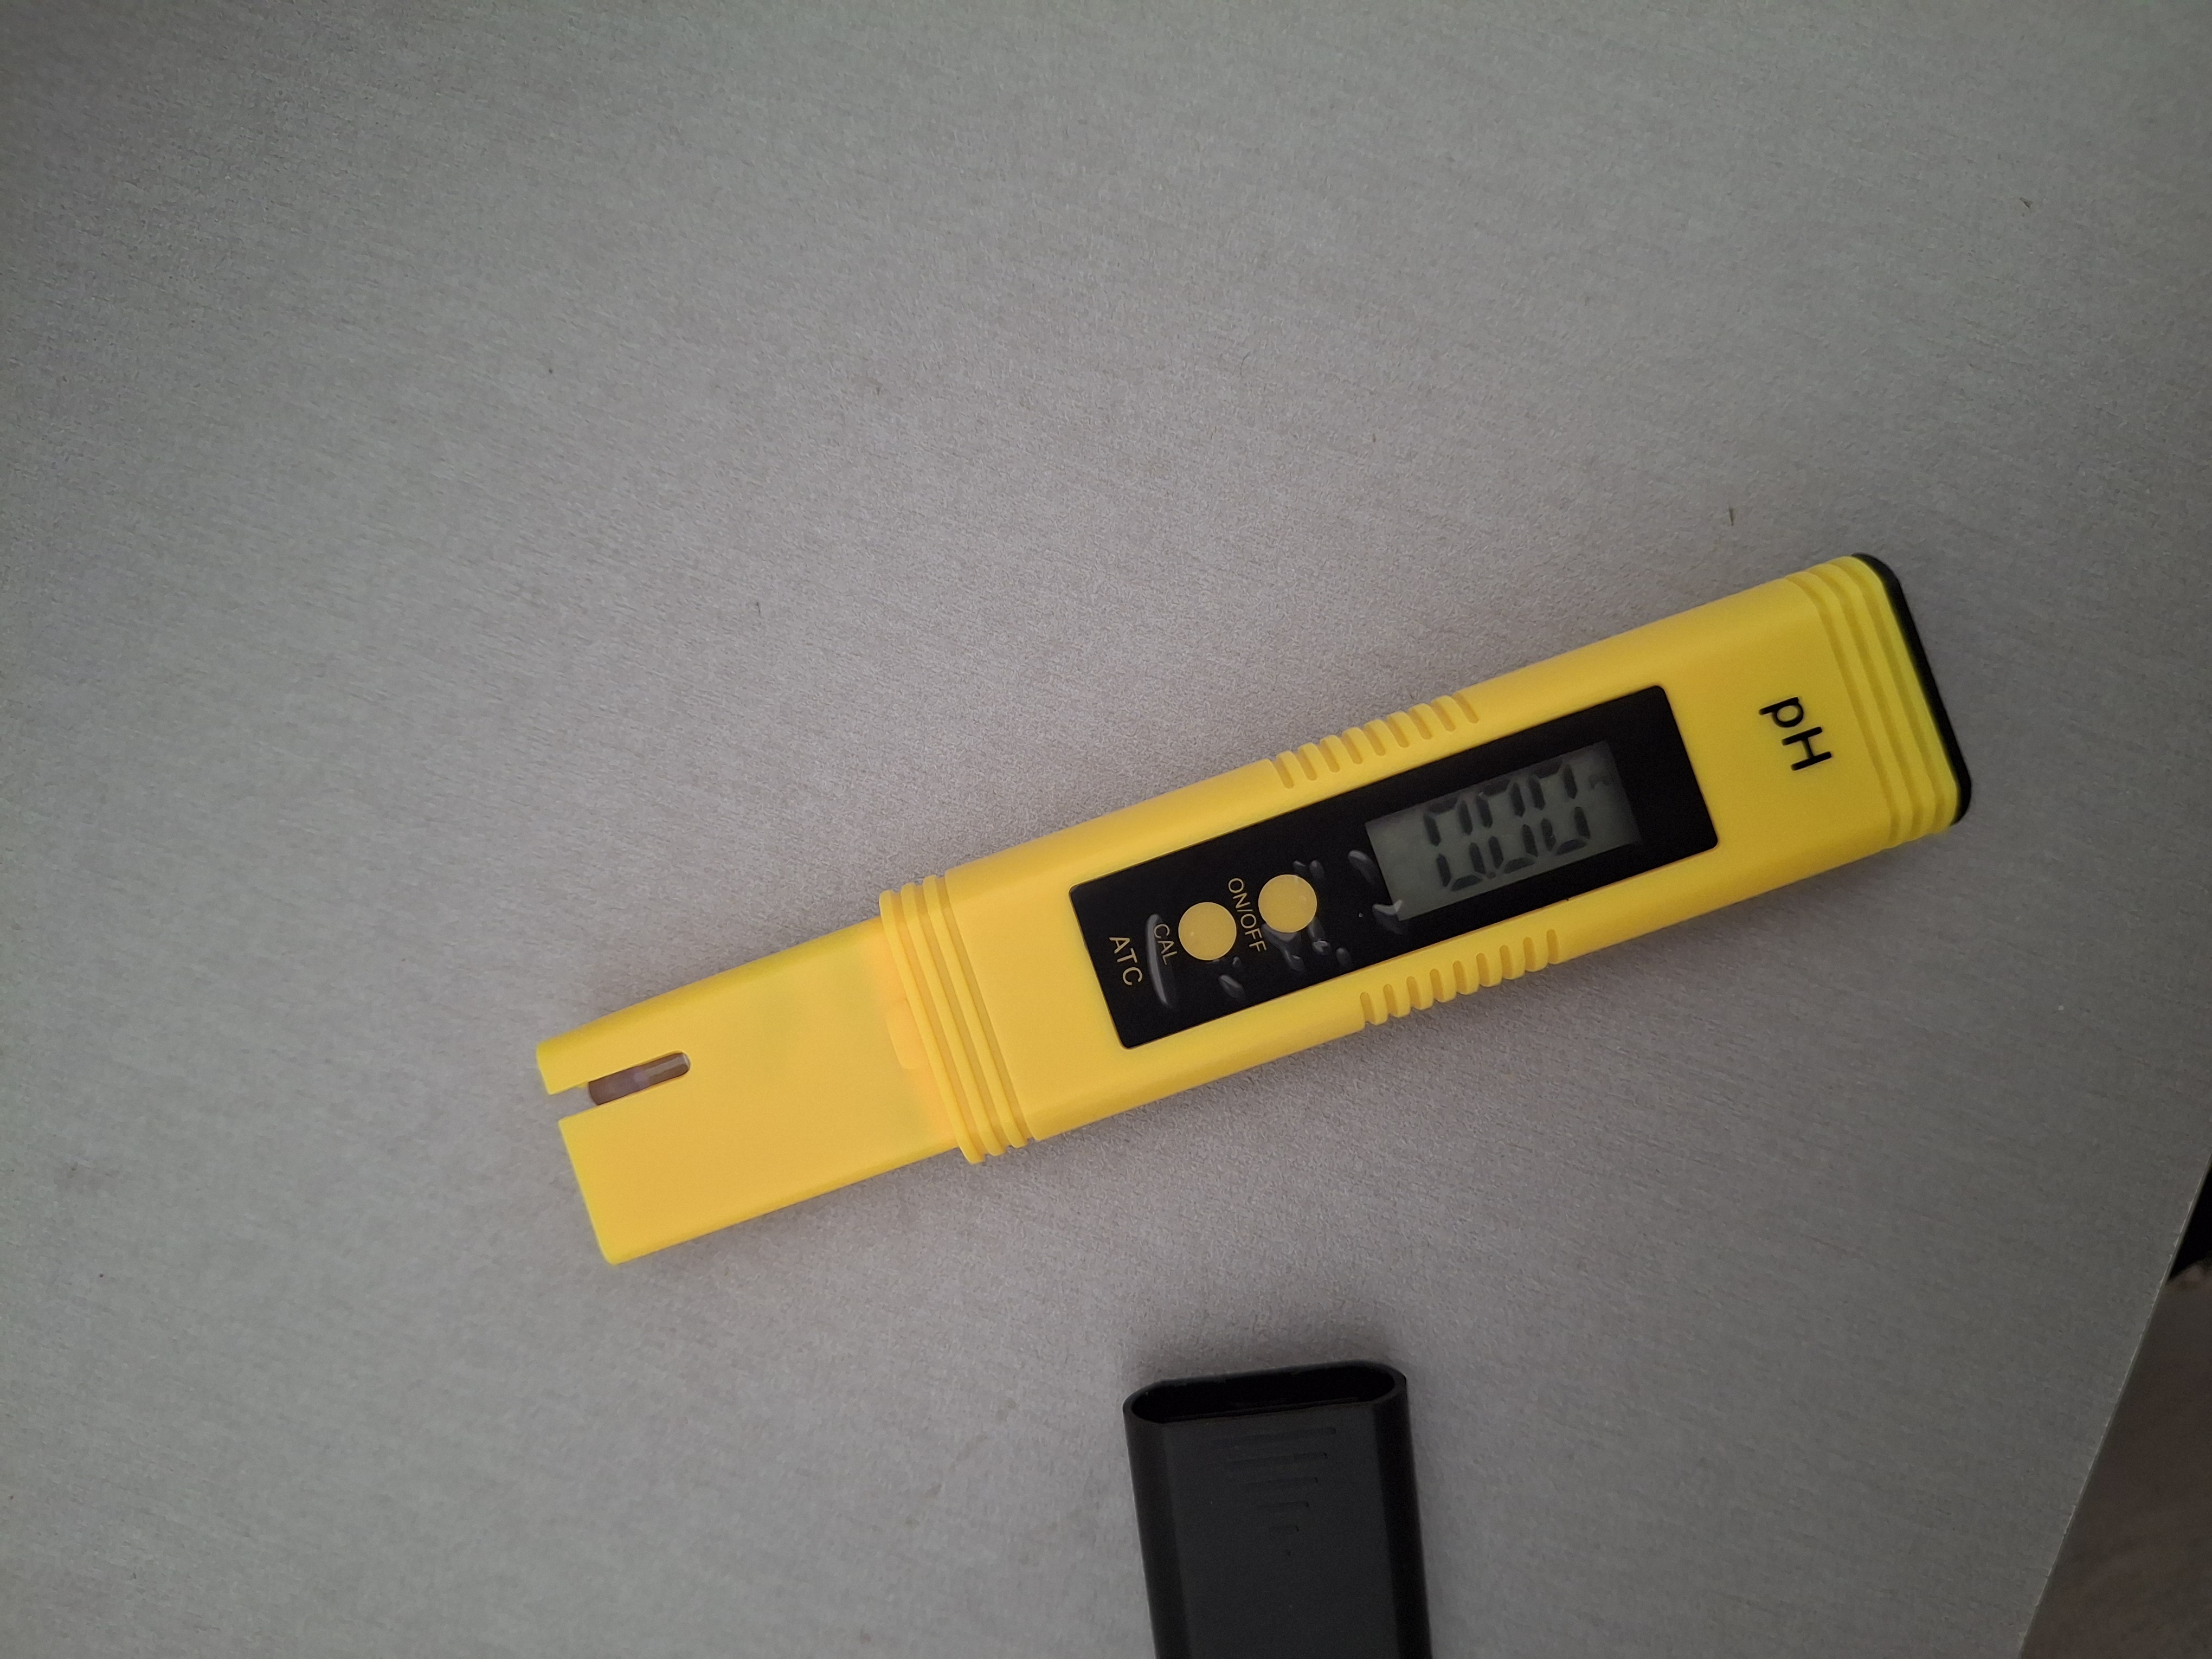
\includegraphics[width=0.5\textwidth]{./Figures/mesurador.png}
% \caption{Mesurador de pH}
% \label{fig:fotoMesuradorPH}%%%Els labels han de ser tots diferents.
% \end{figure}

\begin{minipage}[h]{0.6\textwidth}
\item El TetraTest de Nitrit cedit pel centre. El TetraTest de nitrits és un test químic que permet mesurar la concentració de nitrits (NO$_2^-$) en una mostra d’aigua. Per fer la prova, s’afegeixen unes gotes del reactiu específic a una petita mostra d’aigua, i després d’uns minuts, el color resultant s’ha de comparar amb una escala per determinar la quantitat de nitrits en mg/L.
\end{minipage}
\begin{minipage}[h]{0.35\textwidth}
\begin{figure}[H]
\centering
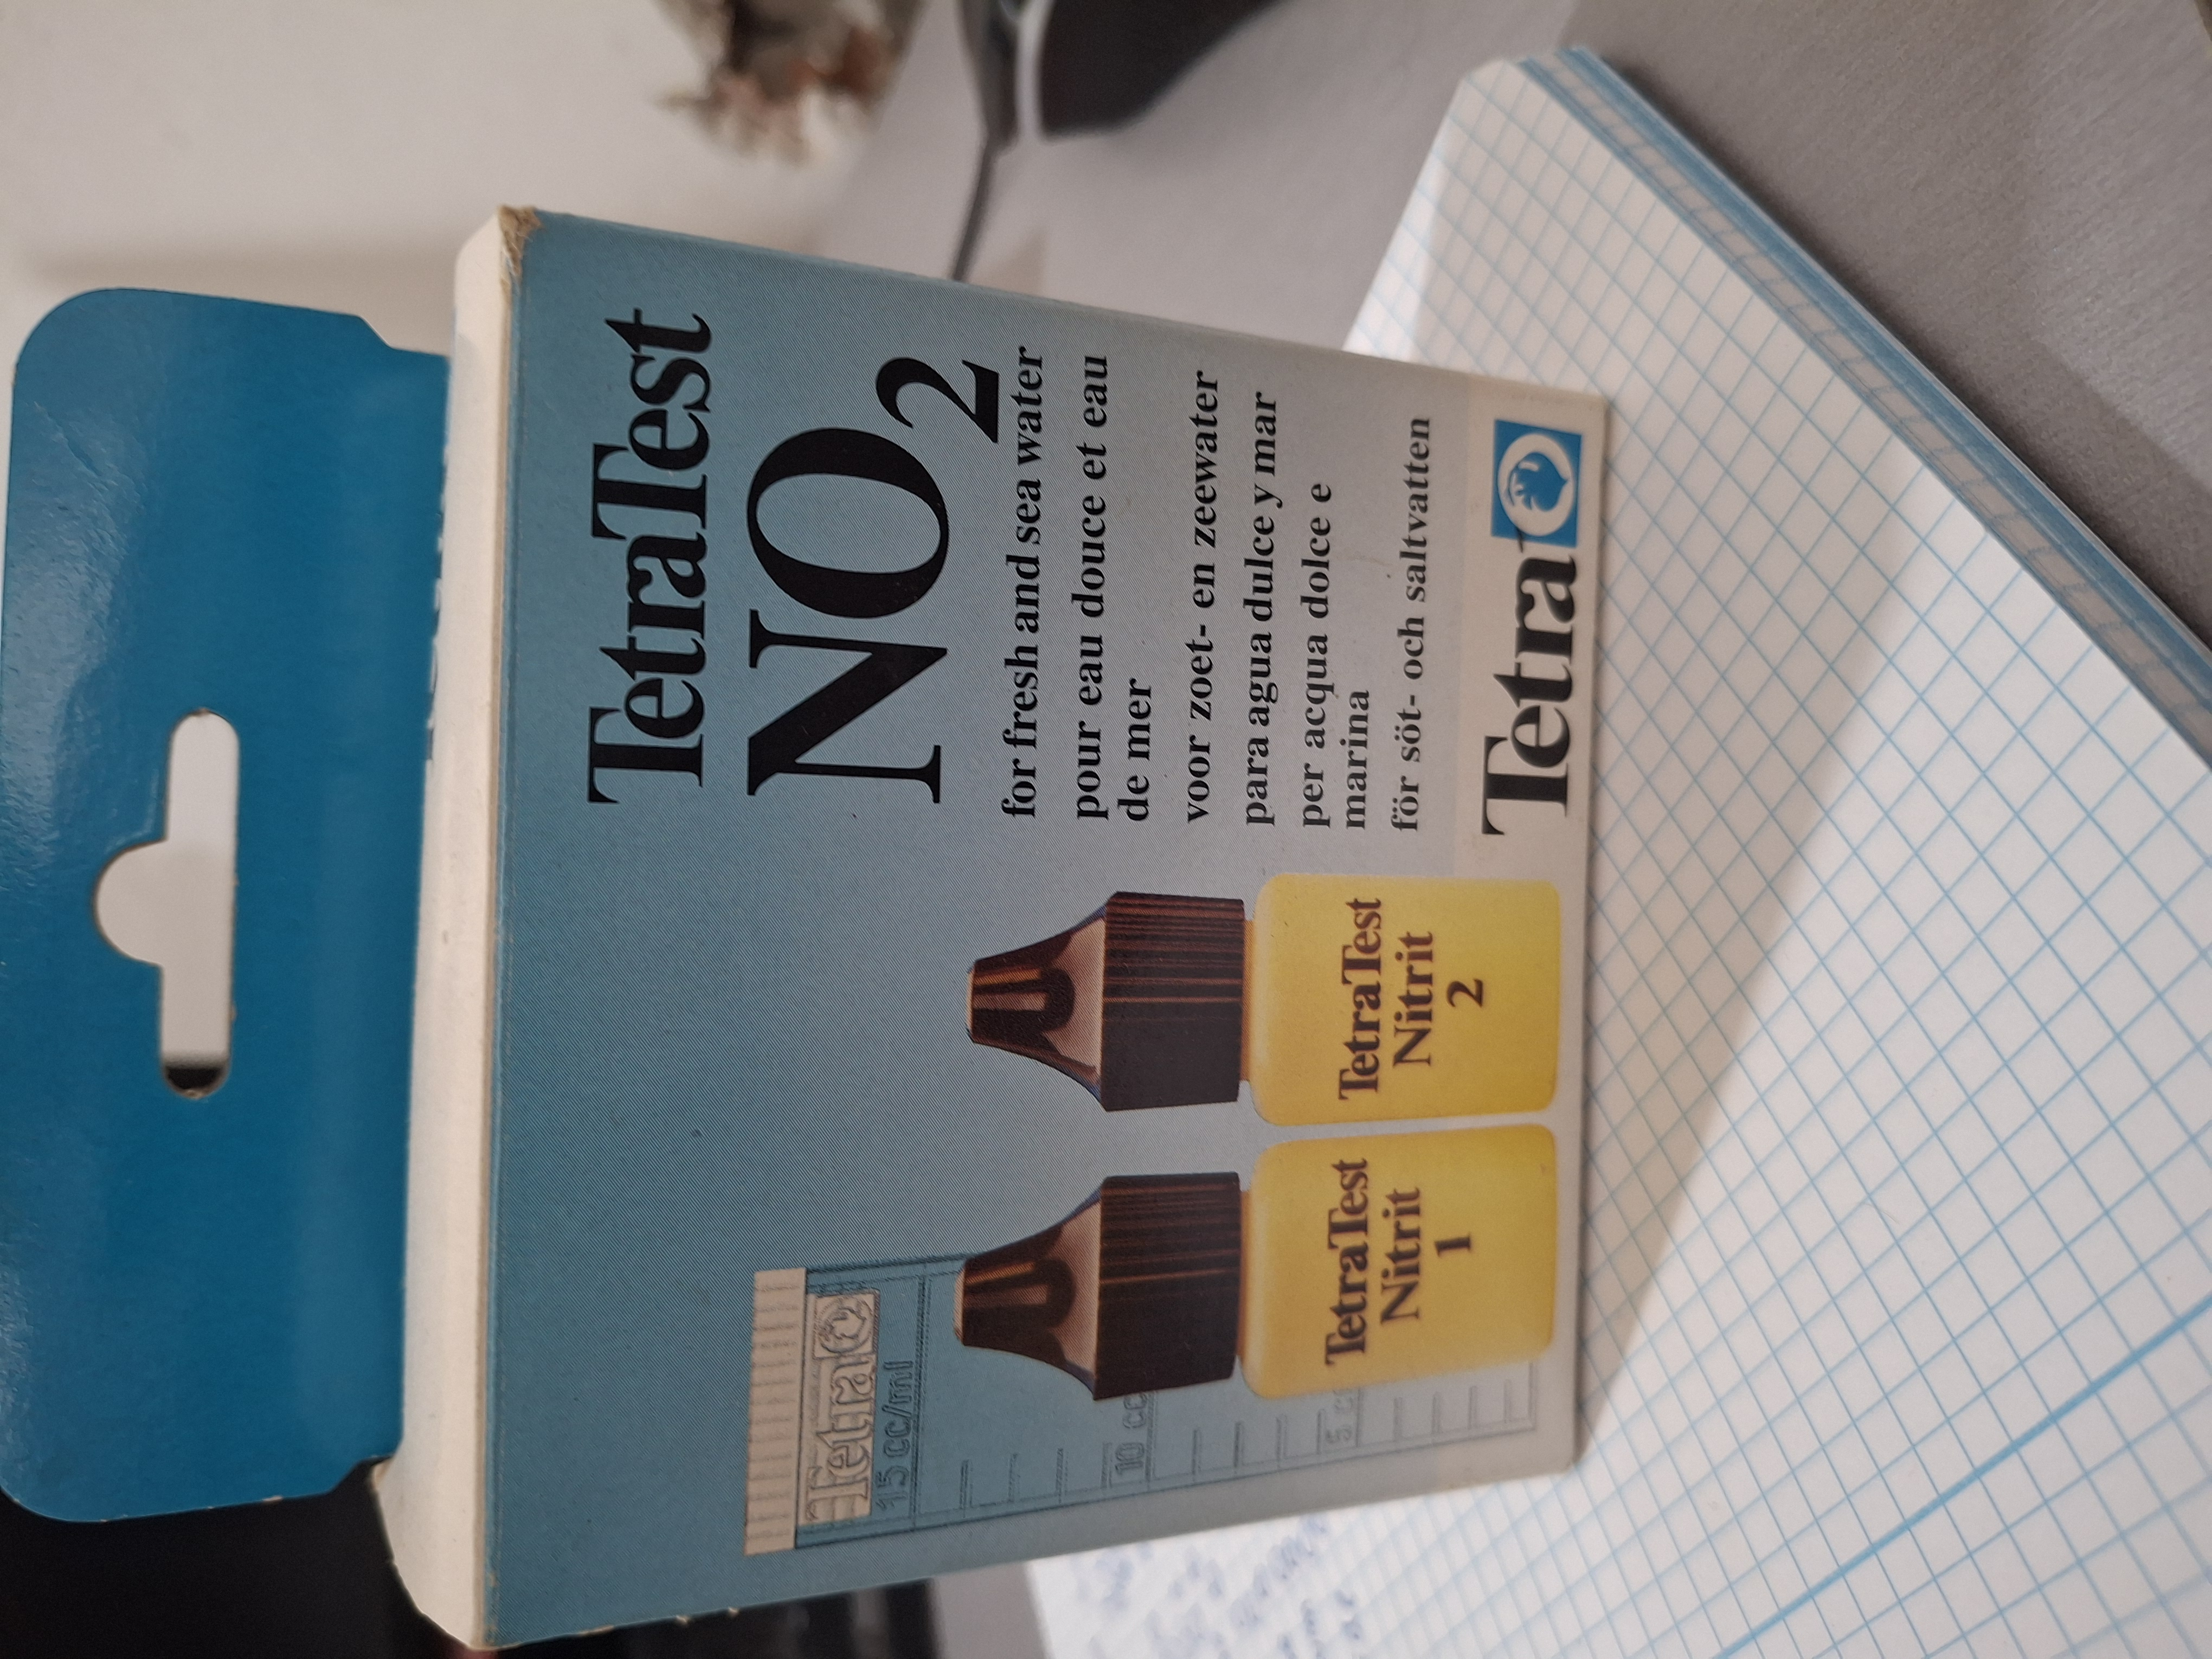
\includegraphics[width=1\textwidth, angle=270]{./Figures/TetraTest.png}
\caption{TetraTest}
\label{fig:TetraTestdeNitrit}
\end{figure}
\end{minipage}

 \item Aigua destil·lada per netejar el mesurador. L’aigua destil·lada és aigua que s’ha purificat per evaporació i condensació, eliminant així sals, minerals i altres impureses.

 \item Un ordinador amb connexió a internet per a comparar les dades obtingudes amb les de la pagina web d'Aigues de Barcelona \cite{qualitatAigua}

 \item Mostres d'aigua. La mostra de la figura~\ref{fig:fotoAiguaCasaMeva} correspon al primer experiment, en aquest cas una mostra d'aigua de casa meva.
 \begin{figure}[h!]
    \centering
    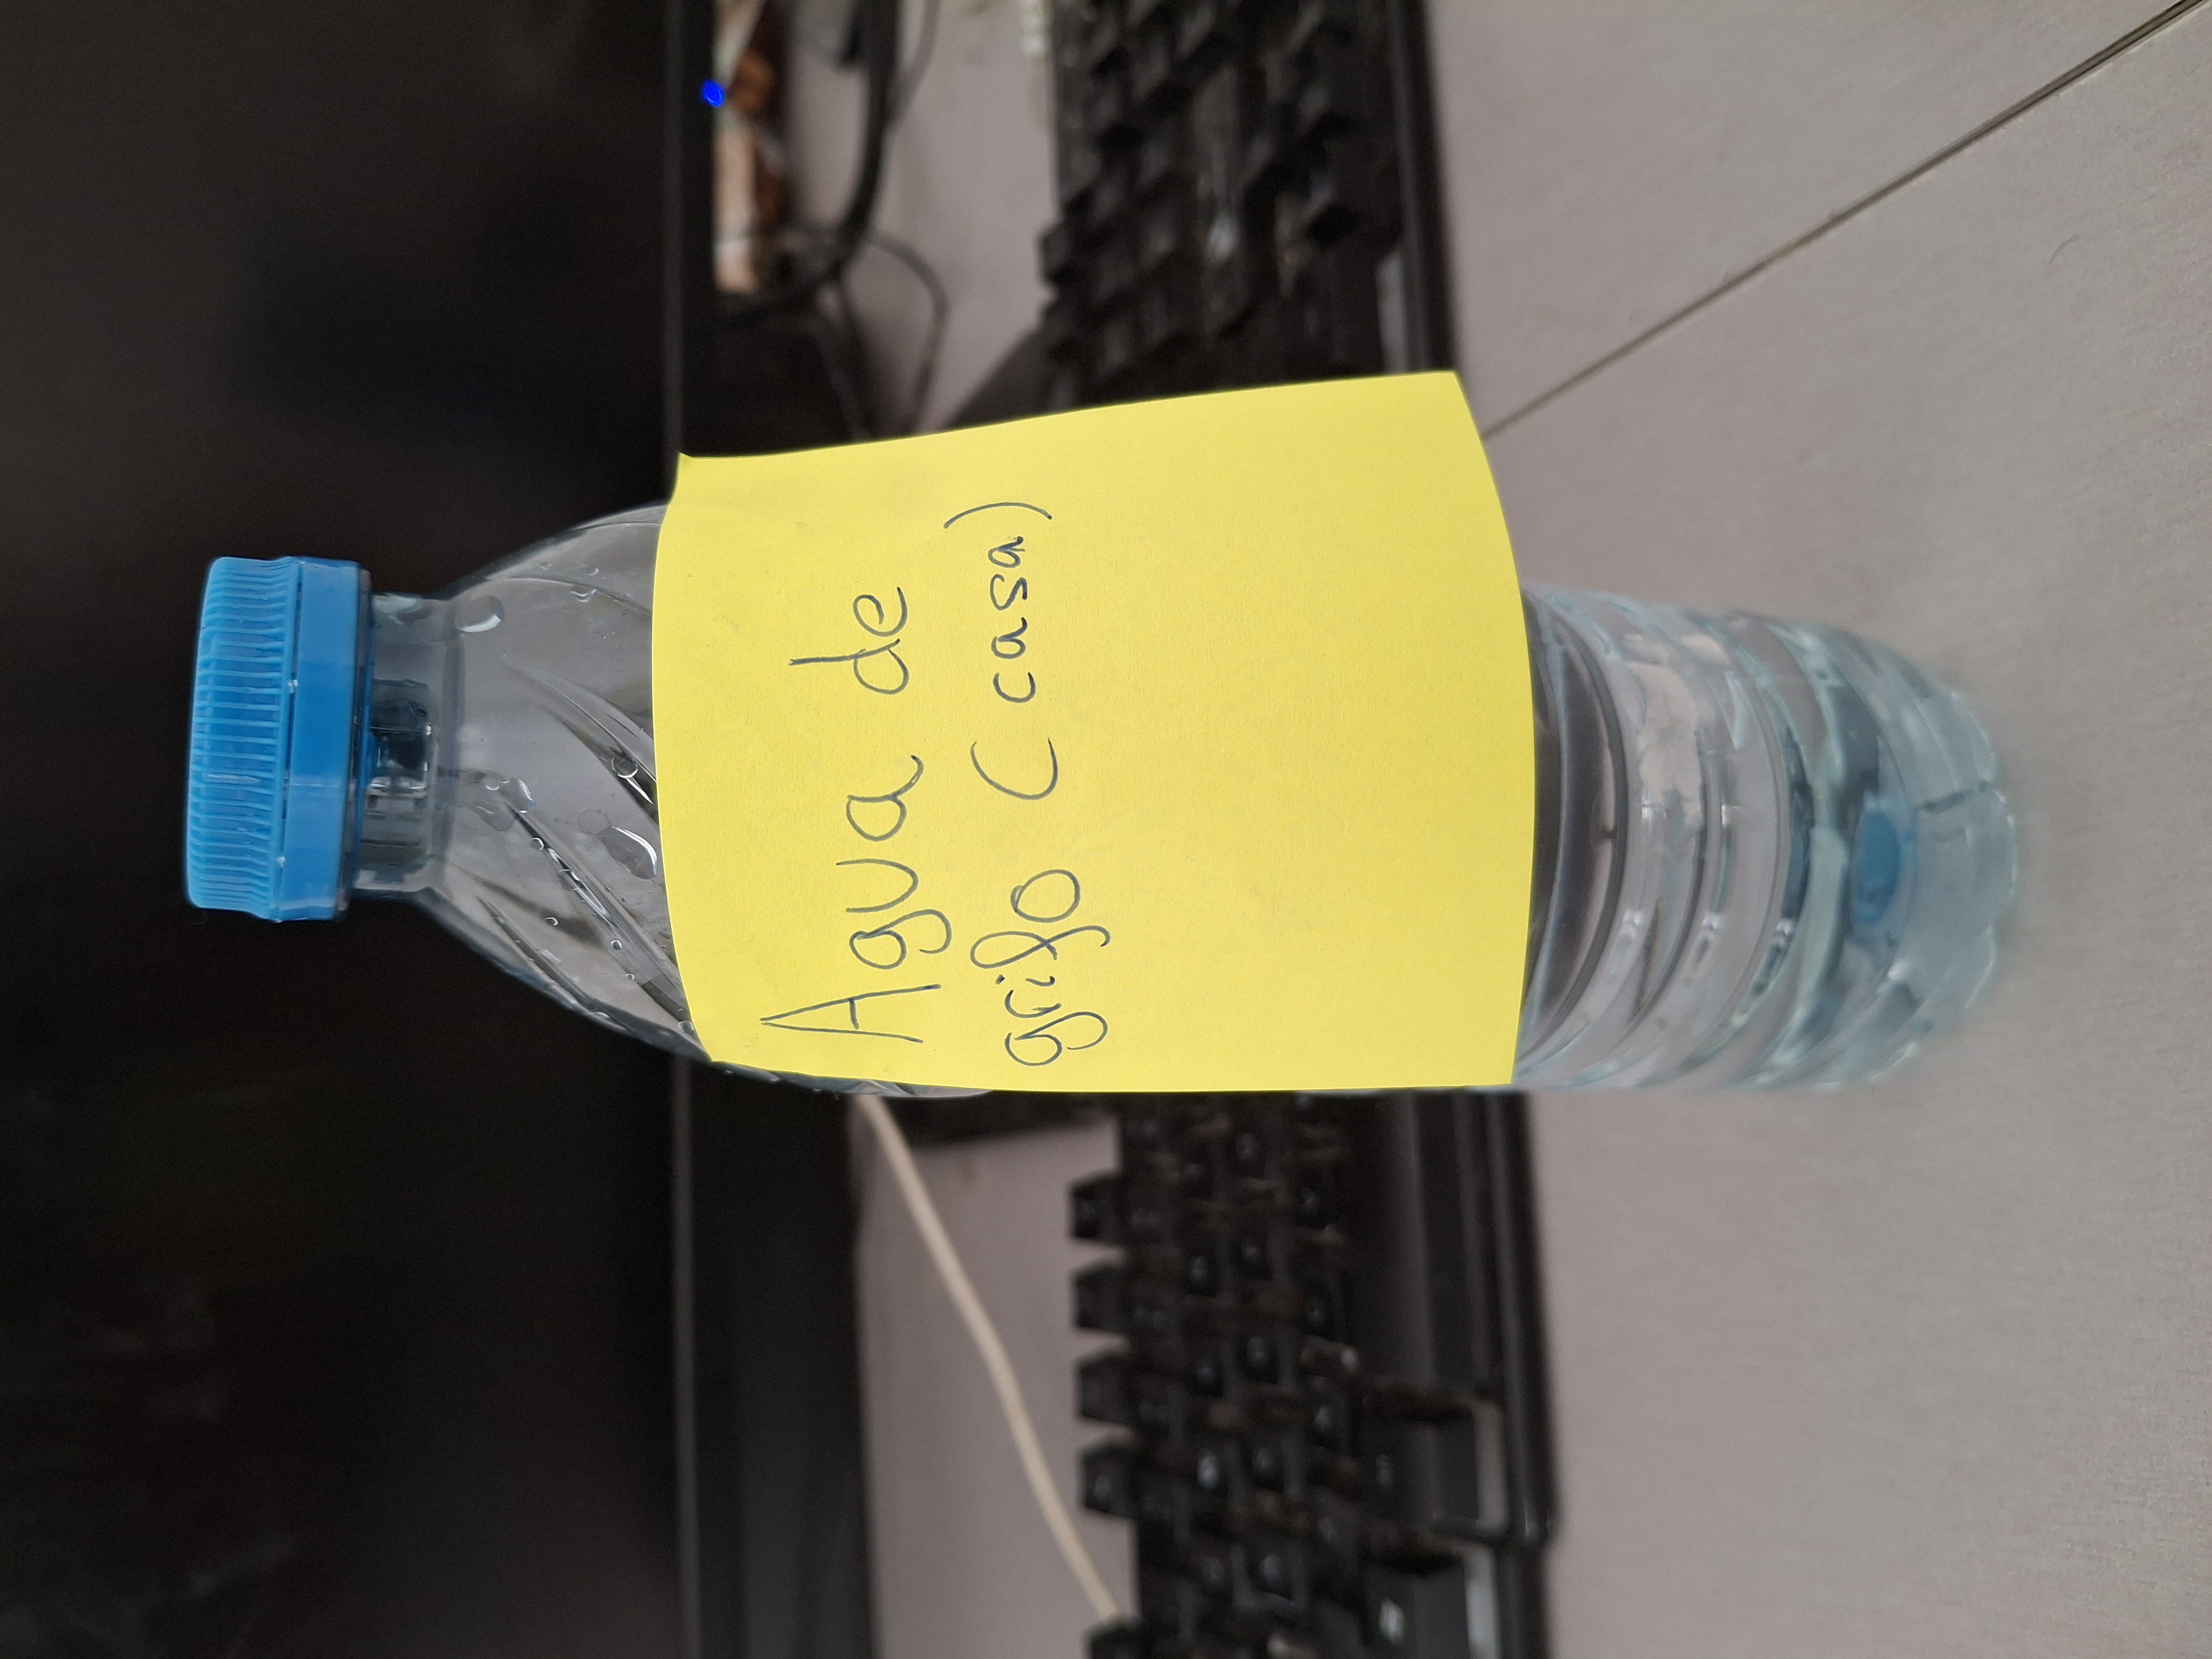
\includegraphics[width=0.4\textwidth, angle=270]{./Figures/aguadecasa.png}
    \caption{Aigua de casa meva}
    \label{fig:fotoAiguaCasaMeva}
  \end{figure}
\end{enumerate}



%%%%%%%%%%%%%%%%%%%%%%%%%%%%%%%%%%%%%%%%%%%%%%%%%%%%%%%%%%%%%%%%%%%%%%%%%%%%%%%%%%%%%%5



% Dono per finalitzada la part de metodologia del treball. He explicat molt per sobre els conceptes i he intentat comprimir al màxim les explicacions, perquè, com bé es pot intuir, el tema de la informàtica és molt ampli. No vull allargar gaire aquesta part, però hi ha molta més informació als \textbf{[aquí posaré una referència als annexos on amplio una mica més el tema de la metodologia]}.
%
% Allà podreu informar-vos una mica més sobre informàtica per entendre millor el tema.
